En una actividad de diseño, se sombrea una región que corresponde a un sector circular de $90^\circ$ dentro de un círculo de radio 4 cm.

\begin{center}
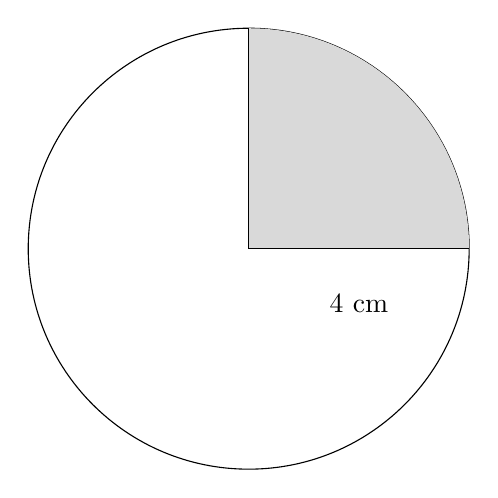
\begin{tikzpicture}[scale=0.7]

% Círculo
\draw (0,0) circle (4);

% Sector sombreado
\fill[gray!30] (0,0) -- (4,0) arc[start angle=0,end angle=90,radius=4] -- cycle;

% Radios
\draw (0,0) -- (4,0);
\draw (0,0) -- (0,4);

\node at (2,-1) {4 cm};

\end{tikzpicture}
\end{center}

¿Cuál es el área de la región sombreada?

\begin{multicols}{2}
\begin{enumerate}[label=\alph*), leftmargin=*]
\item $4\pi$
\item $8\pi$
\item $16\pi$
\item $2\pi$
\end{enumerate}
\end{multicols}